\iffalse METRICS
- Numerical stability of different conformal mapping methods
- Boundary discretization requirements (how smooth does $\gamma$ need to be?)
- Mesh quality preservation - how does the mapping affect triangle quality?
- Computational complexity
- Input and output formats
- https://www.desmos.com/calculator/g9asjc6xph
\fi
\section{Existing Methods}
This chapter aims to give an overview and compare existing methods in terms of input/output format, suitability/ boundary requirements, computational complexity, numerical stability and mesh quality preservation/ accuracy.

We give an overview of some existing methods and how to choose each depending on the application before explaining each of them in more detail.
% THIS SHOULD GIVE A COMPREHENSIBLE OVERVIEW OF POTENTIAL METHODS AND HOW TO CHOOSE THEM
\begin{center}
    \red{maybe change to first boundary smooth then BIE, if not smooth then at least piecewise continuous then SCE, else if not well-behaved IDK}
\begin{tikzpicture}[node distance=1cm]

\node (BVP) {BVP};

\node (Q_poly) [below=of BVP] {$\Omega$ a polygon?};

\node (SCE) [right=of Q_poly] {Schwarz-Christoffel};

\node (Q_BIE) [below=of Q_poly] {Reformulate as BIE?};

\node (Q_star) [below=of Q_BIE] {$\Omega$ star-shaped?};

\node (theo) [below=of Q_star] {Theodorsen's Equation};

\node (BIE) [right=of Q_star] {General BIE Methods};
\node (kerz) [below=of BIE] {Kerzman-Stein};
\node (neu) [below left=of kerz, xshift=1cm] {Neumann Kernel};
\node (symm) [below right=of BIE] {Symm's Equation*};
\node (amano) [below=of symm] {Amano's Method};

\node (other) [right=of Q_BIE] {Other Method Families};
\node (zip) [above right=of other] {Zipper};
\node (berg) [right=of other] {Bergman Kernel};
\node (AP) [below right=of other] {Alternating Projections};

\draw [->] (BVP) -- (Q_poly);

\draw [->] (Q_poly) -- (SCE) 
    node [midway, above] {Yes};
\draw [->] (Q_poly) -- (Q_BIE) 
    node [midway, left] {No};

\draw [->] (Q_BIE) -- (Q_star) 
    node [midway, left] {Yes};
\draw [->] (Q_star) -- (theo) 
    node [midway, left] {Yes};
\draw [->] (Q_star) -- (BIE) 
    node [midway, above] {No};

\draw [->] (BIE) -- (kerz);
\draw [->] (BIE) -- (neu);
\draw [->] (BIE) -- (symm);
\draw [->] (BIE) -- (amano);

\draw [->] (Q_BIE) -- (other) 
    node [midway, above] {No};

\draw [->] (other) -- (zip);
\draw [->] (other) -- (berg);
\draw [->] (other) -- (AP);

\end{tikzpicture}
\end{center}
*(Linear Fredholm $1^{st}$ kind, generally ill-posed -> not preferred)


\subsection{Preprocessing}
\subsubsection{Osculation Methods}

\subsection{Alternating Projections Method}\label{APMethod}
Various methods for numerical construction of $\psi$ essentially construct two sequences of functions, one of normalized analytic functions on the disk (using the operator K \ref{operatorK_N}) and one mapping the boundary of $\disk$ to the boundary $\Gamma$.
The method of alternating projections uses both these sequences and alternates between them to find $\psi$ \cite{Wegmann1989_alternating_projections}.

\red{MOVE THIS TO THE BEGINNING OF THE ARTICLE For this method we suppose $\Gamma=\del\Omega$ is a smooth Jordan curve parametrized by a $2\pi$-periodic function $\eta(s)$ with continuous non-vanishing derivative $\eta'(s)\neq0$ having winding number $1$ on $[0,2\pi)$, i.e. $\Gamma$ surrounds $\Omega$ exactly once.}
\subsubsection{Alternating Projections à la von Neumann} \label{chap:AlternatingProjections}
For two closed convex sets $P,Q$ in a Hilbert space $H$, the method of alternating projections constructs a sequence $(x_n)_n$ as follows: Starting from an arbitrary point $x_0 \in H$, we define 
$$x_{n+1} := \begin{cases}
    \Pi_P (x_n) & n \equiv 0 (\text{mod } 2) \\
    \Pi_Q (x_n) & n \equiv 1 (\text{mod } 2)
\end{cases}$$ 
where $\Pi_P(z)=\min_{x\in P} \| x-z \|^2$ and $\Pi_Q(z)=\min_{x\in Q} \| x-z \|^2$ denote the orthogonal projections onto the sets $P$ and $Q$ respectively.
It can be shown that the sequence $(x_n)_n$ converges in norm to a point tuple $(x*,y*)$ satisfying 
$$
\begin{cases}
    x*=\Pi_P(y*), \\
    y*=\Pi_Q(x*), \\
    d_H(x*,y*)= min_{(x,y)\in P\times Q} \| x-y \|^2
\end{cases}
$$

In particular, $x*=y*$ if $P\cap Q \neq \emptyset$. \cite{Braun2023_AltProjections}

This exact idea is now applied to function spaces:

\subsubsection{Algorithm}
\begin{algorithm}
    \caption{AP-Method}
    \begin{algorithmic}
    \STATE Start with a function $U_0\in W_{\R}$.
    \STATE Given $U_k$ for $k\geq 0$,
        \FOR {$n = 1,0,-1,-2,...$}
            \STATE $a_n = \frac{1}{2\pi}\int_{0}^{2\pi} \eta(t+U_k(t))e^{-int} dt$ \hfill [Calculate Fourier coefficients]
        \ENDFOR
    \STATE $U_{k+1}(t) := U_k(t) - \text{Re}\frac{i (\text{Im}(a_1))e^{it}+\sum_{n=-\infty}^{0} a_n e^{int}}{\dot{\eta}(t+U_k(t))}$ \hfill [Calculate the new iterate]

    %continue here
    \end{algorithmic}
\end{algorithm}

\subsection{Schwarz-Christoffel Method}
\iffalse
$R_w = \mathbb{D}$ disk \\
$B_w = \del\mathbb {D}$ boundary of D\\
$R_z = \Omega$ = polygon \\
\fi 

One class of methods for finding the conformal mapping $\Phi$ is given by the Schwarz-Christoffel equation, which relates the derivative of $\Phi$ to an integral over the boundary of the target domain $\Omega$ when $\Omega$ is a polygon.
\subsubsection{Preliminaries and Notation}
\begin{definition}
    A \textbf{Polygon} is a planar figure whose boundary is made of a chain of connected line segments which we will call arcs, connecting corner points.
\end{definition} 

The unit disk $\mathbb{D}$ is in particular a polygon, and we parametrize the boundaries $\del\mathbb{D}$ and $\del\Omega=\Gamma$ by collections of arcs $s_{\mathbb{D}}$ and $s_{\Omega}$ respectively, in positive mathematical orientation. 
These arcs being smooth yields tangents with well-defined derivatives at every point of the boundary curves except for corners, and we denote the angles of these tangents with $\theta_{\mathbb{D}}(s_{\mathbb{D}})$ and $\theta_{\Omega}(s_{\Omega})$ respectively. If $z_0$ is a corner it will have a turning angle of 
$$\measuredangle\theta_{\mathbb{D}}(z_0)=\theta_{\mathbb{D}}(z_0+\eps)-\theta_{\mathbb{D}}(z_0-\eps),$$ 
where $\eps\to0$. The same applies to corners of $\Omega$. Then,
$\frac{\del\theta_{\mathbb{D}}}{\del s_{\mathbb{D}}} = \measuredangle\theta_{\mathbb{D}}(z_0)\delta(s_{\mathbb{D}}-z_0)$ for $\delta$ the Dirac function, and similarly for $\theta_{\Omega}$ and thus $\theta_{\mathbb{D}}$ and $\theta_{\Omega}$ are piecewise continuously differentiable functions with jump discontinuities at the corner points.

\red{\subsubsection{the log derivative of Phi}}

\subsubsection{Green's Functions}
A Green's function is a general concept for solving differential equations containing a linear operator.
\begin{definition} 
    A \textbf{Green's function} or \textbf{Green function $G(x,s)$} is any solution to $$LG(x,s)=\delta(x-s)$$ where $L=L(x)$ is a linear operator acting on distributions over $\R^{n}$ and $\delta$ is the Dirac delta function.
\end{definition}
This definition can be exploited to solve inhomogeneous differential equations of the form $Lu=f(x)$.
In the case of the SCE the Green's function are defined as $G(z,z'):\mathbb{D}\to\mathbb{R}$ satisfying $$\nabla^2 G(z,z') = 2\pi \delta(u-u')\delta(v-v') $$ inside the disk and $$\frac{\del G(z_B, z')}{\del n} = \beta_i$$ where $n$ is the outward normal vector at the boundary point $z_B \in \del\mathbb{D}$ and $\beta_i$ is a real constant associated with the $i$'th arc's length $l_i$ such that $\sum l_i\beta_i = 2\pi$. It can be shown according to Floryan and Zemach that this defines a unique Green's function up to an additive constant \cite{FLORYAN1987_SC_general}.
The SCE can be written explicitly whenever the Green's function is \red{obtainable in closed analytic form, i.e. expressable via a finite number of elementary operations (is that what is meant on p348? i looked up wikipedia for closed analytic form)}.

\subsubsection{Schwarz-Christoffel Equation Variants}
Let $\mathcal{G}(z, z_B')$ be a complex extension of the above defined $G(z,z_B')$, i.e. $\mathcal{G}(z, z_B')$ is analytic with real part $G(z,z_B')$.
A Schwarz-Christoffel equation for a conformal mapping $\Phi(z):\mathbb{D}\to\Omega$ has the form $$ log \frac{d\Phi}{dz}= C+\displaystyle\sum_i Q_i,$$ where $C\in\mathbb{C}$ is a constant and the $Q_i$ are the Green's function integrals over the boundary arcs of $\mathbb{D}$.
Some parameters and constants have to be determined in order to get a unique $\Phi$ for a particular given $\Omega$. The Riemann mapping theorem allows \red{HOW?} for the first three real parameters to be preassigned, for example to three boundary points in the case of simply connected bounded $\Omega$. The remaining degrees of freedom must be solved for using properties of the arcs $s_{\Omega}(s_z)$ and $s_{\mathbb{D}}(s_z)$. 

The most general form is called Schwarz-Christoffel equation with subtraction \cite{FLORYAN1987_SC_general}:
$$log(\frac{d\Phi}{dz}) = C_0 - \frac{1}{2\pi}\displaystyle\int_{\del\mathbb {D}} [\mathcal{G}(z, z_B')-\mathcal{G}(z_0, z_B')] \times [d\theta_{\Omega}(s_z')-d\theta_{\del\mathbb{D}}(s_z')]$$
where $C_0\in\mathbb{C}$ is a constant, $z_0$ is a fixed point in $\mathbb{D}$\red{or del?}, $\mathcal{G}(z,z_B')$ is the fundamental solution of the Laplace equation in $\del\mathbb{D}$ with singularity at $z_B' \in \del\mathbb{D}$\red{not at the boundary of omega?}. However, we can use an unsubtracted form of this equation since the integrals converge separately and we know our $\Omega$ is bounded (hence we need not care about behaviours at infinity), yielding the simpler form
$$log(\frac{d\Phi}{dz}) = C - \frac{1}{2\pi}\int_{\del\mathbb{D}} \mathcal{G}(z, z_B') [d\theta_{\Omega}(s_z')-d\theta_{\del\mathbb{D}}(s_z')]$$

\subsubsection{Implementation}
\cite{Brown1990_SC_meshgen}
\cite{Trefethen1980_SCnumericalcomputation}
\cite{banjaitrefethen2006_SCmultipolemethod}
\cite{Bezrodnykh2022_lauricella}
Crowding is a problem because it yields exponential derivative of $\Phi$, but can be fixed. \cite{Banjai2008_SC_crowdingworkaround}

\subsection{Zipper Method}
This algorithm was fonud independently by Kühnau and Marshall in the 1980's has the advantage of finding $\Phi$ and its inverse at the same time. 
The computed map is only approximately conformal, and is obtained as a composition of conformal maps onto slit halfplanes. Depending on the shape of the slits, the Zipper algorithm looks a bit different. 
In this section we will focus on the easiest version called the "geodesic algorithm" \cite{marshall2006_convergencezipperalgorithmconformal} which is quite beautiful from a geometric perspective.
\subsubsection{The Geodesic Algorithm}
The most elementary version of this algorithm is based on a function 
$$f_a: \mathbb{H}\setminus \gamma \to \mathbb{H}$$
where $\mathbb{H}$ is the upper half plane and $\gamma$ is a circular arc from $0$ to $a\in\mathbb{H}$ which is orthogonal to the real axis. The orthogonal circle also meets the real axis again at $b=|a^2|/Im(a)$. Then the map can be expressed in closed form as 
$$f_a(z) = \sqrt{g_a \circ h_a (z)}$$ where $g_a(z) = z^2 + c^2$ and $h_a(z) = \frac{z}{1-z/b}$.

\red{INSERT IMAGE}

Now suppose $z_0, z_1, ..., z_n$ are points arranged counterclockwise on a Jordan curve $\Gamma$ in the upper half plane. The geodesic algorithm basically iterates over the arcs from $z_i$ to $z_{i+1}$ and "unzips" them one by one using the map $f_{a_i}$ where $a_i$ is the image of $z_{i+1}$ under the composition of all previous maps.
\red{The original geodesic algorithm proposed by Marshall and Rohde constructs a conformal map from the upper half plane to the region bounded by $\Gamma$, but it can be adapted to map from the unit disk as well via a Möbius transformation mapping the half plane to the unit disk and back first (hopefully?).}

\begin{algorithm}
    \caption{Geodesic Zipper Algorithm}
    \begin{algorithmic}
    \STATE \textbf{Input:} Points $z_0, z_1, ..., z_n$ on a Jordan curve $\Gamma$ in the upper half plane.
    \STATE \textbf{Output:} $\psi$: conformal map from $\mathbb{H}$ to the region bounded by $\Gamma$ and its inverse $\psi^{-1}$.
    \STATE $\phi_1(z) := i\sqrt{(z-z_1)/(z-z_0)}$
    \STATE $\zeta_2:= \phi_1(z_2)$
    \STATE $\phi_2(z) := f_{\zeta_2}(z)$
    \FOR{k in n}
        \STATE $\zeta_k := \phi_{k-1} \circ \ldots \circ \phi_1 (z_k)$
        \STATE $\phi_k(z) := f_{\zeta_k}(z)$
    \ENDFOR
    \STATE Finally, $\zeta_{n+1} := \phi_n \circ \ldots \circ \phi_1 (z_{0})\in\R$ and $\phi_{n+1}(z) := -(\frac{z}{1 - z/\zeta_{n+1}})^2$
    \STATE Then $\psi(z) := \phi_1^{-1} \circ \phi_2^{-1} \circ \ldots \circ \phi_{n+1}^{-1}(z)$ and $\psi^{-1}(z) := \phi_{n+1} \circ \ldots \circ \phi_2 \circ \phi_1 (z)$
    \end{algorithmic}
\end{algorithm}
\red{INSERT IMAGE}

\subsubsection{The Slit Algorithm}
The above geodesic algorithm is only as accurate as the approximation of the boundary curve $\Gamma$ by circular arcs between the points $z_i$. A more accurate version is given by the slit algorithm, which uses straight line segments instead of circular arcs.
We therefore exchange the map $f_a$ for a map $g_a: \mathbb{H}\setminus L \to \mathbb{H}$ where $L$ is the line segment from $0$ to $a\in\mathbb{H}$. This map does not have a closed form expression, but can be computed numerically using Newton's method.

\subsubsection{The Zipper Algorithm}
The approximation of $\Gamma$ by circular arcs or straight line segments can be further improved by using circular arcs which meet $\Gamma$ tangentially at the points $z_i$. Each arc is determined by the points $z_i, z_{i+1}$ and $z_{i+2}$, hence we assume an even number of boundary points. 
The first arc is replaced by $$\phi_1(z)=\sqrt{\frac{(z-z_2)(z_1-z_2)}{(z-z_0)(z_1-z_2)}}.$$ At each subsequent step that circular arc through $\zeta_k$ and $\zeta_{k+1}$ is mapped onto a straight line segment by a Möbius transform, and then the Slit Algorithm is applied to unzip that segment.
\red{This yields a sort of "quadratic approximation" of $\del\Omega$ instead of a linear one.}

\red{GOOD PAPER FOR IMPLEMENTATION ESPECIALLY END NOTES}

\subsection{Newton/ Wegmann Method}
For smooth $\del\Omega$, Integral equations of the second kind can also be solved by Newton's method \cite{Wegmann1978_newtonverfahren}.
Let $\eta$ be a differentiable parametrization of $\Gamma$ and $\dot\eta(s)\neq 0\forall s$. 

\iffalse NOT NEEDED SINCE WE ARE ISMPLY CONNECTED
Let $\kappa\geq 1$ be the winding number of $\dot\eta$ with regard to $0$, then we get \red{$\kappa -1$} additional degrees of freedom 
\begin{equation}
\psi_{\red{0}} (z_n) = c_n \quad n=0,1,2,...,\kappa \text{ where } z_0\in\del\disk, z_1, ..., z_{\kappa}\in\disk, c_0 \in\Gamma
\end{equation}to fix for the \red{initial?} interpolation. 
\fi

Let $S(\zeta)$ be a $2\pi$-periodic function such that $\psi(\zeta)=\eta(S(\zeta))$.
$$
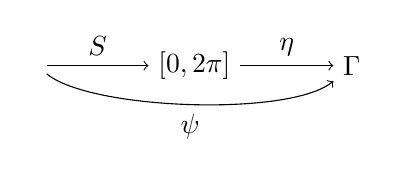
\begin{tikzpicture}[node distance=2cm, auto]
\node (A) {$\disk$};
\node(B) [right of=A] {$[0,2\pi]$};
\node (C) [right of=B] {$\Gamma$};
\draw[->](A) to node {$S$}(B);
\draw[->](B) to node {$\eta$}(C);
\draw[->, out = -40, in = -140, looseness = 0.5] (A) to node [below]{$\psi$}(C); % this should be a circular arrow under the diagram
\end{tikzpicture}
$$
We approximate the conformal map $\psi$ as follows:
%Assume a starting configuration of points $z_1, z_2, ..., z_N$ in $\disk$ and their images $\zeta_1, \zeta_2, ..., \zeta_N$ on $\Gamma$ such that $\psi(z_k)=\zeta_k$. 
Assume that the approximation for $\psi$ after $k$ steps be given by $\psi_k(\zeta)=\eta(S_k(\zeta))$. We improve the approximation by moving the points along the tangent towards the boundary curve, i.e. by finding a correction function $U_k:\del\disk\to[0,2\pi]$ such that
\begin{equation}\label{eq:h_k+1}
    \eta(S_k(\zeta))+U_k(\zeta)\dot\eta(S_k(\zeta)) = h_{k+1}(\zeta)
\end{equation}
where $h$ is analytic on $\overline\Omega$ and $h_{k+1}(\zeta)$ is the boundary value of the next approximation $\psi_{k+1}(z_n)=c_n$.
For the boundary point $z_0$ we are given $c_0=\eta(s_0)\in\Gamma$. Note that since $h_{k+1}(z_0)$ lies on the tangent through $\eta(S_k(z_0))$ we cannot have $h_{k+1}(z_0)=c_0$ unless $\eta(S_k(z_0))=c_0$. Therefore we set
\begin{equation}
    U_k(z_0)=s_0-S_k(z_0).
\end{equation}
Note also that $h_{k+1}$ is an approximation of $\psi$ but it does not generally take values on $\Gamma$. We get an approximation for the parametrization $S$ by $$S_{k+1}(\zeta):= S_k(\zeta)+U_k(\zeta).$$

\subsubsection{Implementation}
Since we assume $\psi$ to map from the unit disk $\disk$, the integral equations can be explicitly solved by discretization and trigonometric interpolation:
Take $N=2n$ equidistant points $\zeta_k=e^{i\theta_k}$ on the boundary of the disk, where
$$\theta_k = \theta_0 + \frac{\pi k}{n}, \quad k\in[2n-1]$$
and write the integrals in terms of their Fourier transform
\begin{equation}
    F(z)=\frac{1}{2\pi i}\int \frac{\sigma_n(\zeta)}{\zeta - z} d\zeta
\end{equation}
where $\sigma_n(\zeta_k)=\sum_{i=-n}^{n} c_k \zeta_k^i$. This can be computed fast ($\in\bigO(n\log n)$) via FFT.
% Then, given $\eta(s)$, $\dot\eta(s)$ and $\Theta(s):= arg(\dot\eta(s))$ in closed form, and given initial values $S_1(\zeta_k)$ the next iteration is computed as follows:
Each iteration is computed via interpolating polynomials.


\subsection{Theodorsen's Method} \label{TheodorsenMethod}
% \cite{Song2012_theodorsen_equation}
\red{probably put this before wegmann method}

We can reformulate the problem of finding the conformal mapping $\psi:\disk\to\Omega$ as solving Theodorsen's integral equation for the boundary correspondence function $\theta(s)$ \red{rename theta to S?} defined by 
\begin{equation}
    \psi(e^{is})=\eta(\theta(s)) \text{ and } \int_{0}^{2\pi} \theta(s) ds = 2\pi^2
\end{equation} where $\eta$ is a parametrization of $\Gamma=\del\Omega$.
$\psi$ is assumed to be normsalized such that $\psi(0)=0$ and $\psi'(0)>0$.
Theodorsen's integral equation states that $Y:s\mapsto \theta(s)-s$ is  the conjugate periodic function of $X:s \mapsto \log(\eta(\theta(s)))$.
After discretization, Theodorsen's integral equation becomes the fixed point equation
\begin{equation}\label{eq:TheodorsenDiscretized}
    y=\Psi(y):=K_{\Sigma} \log(\eta(s+y))
\end{equation} for $s:=(\frac{k\pi}{N})_{k\in[2N-1]}$ where $y$ approximates $Y(s)$.
The product $y$ can be computed efficiently using FFT (see \ref{operatorK_N}).
If the discretization is based on trigonometric interpolation, $K_{\Sigma}$ is called \textbf{Wittich's matrix} \cite{Gutknecht1983_theodorsen_equation_FFT}.
By a permutation $P$ the above components can be brought to the form
\begin{equation}
    PK_{\Sigma}P =
    \begin{pmatrix}
        0 & -L^T \\
        L & 0
    \end{pmatrix}, \quad
    Py = \begin{pmatrix}
        y^{"} \\
        y^{' }
    \end{pmatrix}, \quad
    Ps = \begin{pmatrix}
        s^{"} \\
        s^{'}
    \end{pmatrix}.
\end{equation}
By Niethammer, (\ref{eq:TheodorsenDiscretized}) can be solved using nonlinear successive over-relaxation (SOR) for given $y_0^{"}, y_0^{'}$ and $\omega$ (relaxation factor) and $m\geq 0$:
\begin{equation}\label{eq:SOR}
    \begin{matrix}
        y_{m+1}^{"} &:= &(1-\omega)&y_m^{"} &- &\omega L^T \log(\eta(s^{'} + y_m^{'})) \\
        y_{m+1}^{'} &:= &(1-\omega)&y_m^{'} &+ &\omega L \log(\eta(s^{"} + y_m^{"}))        
    \end{matrix}
\end{equation}
Alternatively, nonlinear Jacobi iteration with relaxation (JOR) can be used:
\begin{equation}\label{eq:JOR}
    \begin{matrix}
        y_{m+1} &:= &(1-\omega)&y_m + &\omega \Psi(y_m).
    \end{matrix}
\end{equation}

In case of $\Gamma$ not being smooth, Theodorsen's method becomes inaccurate \cite{Gutknecht1983_theodorsen_equation_FFT}. In this case, the boundary curve can be smoothed first using preliminary maps \red{see osculation methods}.

Theodorsen's method \ref{TheodorsenMethod} needs $\Omega$ to be star-shaped in order to converge \cite{Wegmann1978_newtonverfahren} and is particularly simple (fixed point equation) in this case.In practice, the star-shape requirement can be relaxed be smoothing the boundary curve first using preliminary maps \cite{Gutknecht1983_theodorsen_equation_FFT}.


% \subsection{Shirokova's Method}
% \cite{Shirokova2014}

\subsection{Conjugate Function Method}
Hakula, Quach and Rasila \cite{Hakula_2013_conjugatefunctionmethod} presented a new method in 2010 which is based on numerical solution of the Laplace equation subject to Dirichlet-Neumann mexed-type boundary conditions by using $hp$-FEM.  
In their paper they construct the mapping starting from a quadrilateral, but it can be tweaked to map from the unit disk as well. 
"It is well known that one can express the modulus of a quadrilateral Q in terms of the solution of the Dirichlet-Neumann mixed boundary value problem [\red{FIND HENRICI'S BOOK}, p. 431]."


\subsection{Amano's Method of Fundamental Solutions}
\cite{Sakakibara2019_AmanosMethod}
\red{jordan region}
\cite{Amano1998_Amanosmethod}

\subsection{Probabilistic Uniformization Method}
In 2007, Binder, Braverman ans Yampolsky proposed a method for finding a conformal map using a random walks solver to the general Dirichlet problem. They conjectured an upper bound of polynomial space and time for an algorithm with precision $\frac{1}{n}$ pixels (for explicitly given $\del\Omega$; quadratic if $\del\Omega$ is given only approximately, via a so-called \textit{oracle}, sort of a Dirac delta function). \cite{binder2007_computationalcomplexityriemannmapping}



\subsection{Comparison}
We can directly rule out some of the options due to our project constraints: 
First we note that Schwarz-Christoffel only works on polygons and Theodorsen's method is restricted to star-shaped regions. For general $\Omega$ as we are interested in, we therefore have to disregard these two methods. \red{put in each method's description what exactly it gets its restriction from, e.g. pinpoint the bottleneck}
The Zipper method seems very well implementable and robust, but we have to fulfill efficient point evaluations of both $\psi$ and its derivative, which is not possible since the Zipper method essentially constructs $\psi$ as a composition of many maps, and \red{I'm not sure this is efficiently derivable}.
We refrain from using probabilistic methods due to their inherent randomness and the difficulty of guaranteeing a certain accuracy.
Amano's Method of Fundamental Solutions seems good for fast point-evaluations of $\psi$ itself, but the derivative could be tricky due to $\psi$'s form. Moreover,we cannot use our Fourier parametrization nor our mesh in this method, so it will probably now be the best choice for our specific problem. Its accuracy and convergence depend on the right choice of charge points, which is another difficulty, especially given the generality of our target domain.
The Conjugate Function Method is very beautiful mathematically, but it relies only on $hp$-FEM for which there already are powerful libraries, so there would not be much value in half-assing an FEM solver given the scope of this thesis. 

On the other hand, the Alternating Projections Method uses our boundary parametrization in its Fourier series form, \red{remains to check efficient point evaluations}
Also, Wegmann's Newton method seems very promising since it can be implemented efficiently using FFT and also uses our Fourier parametrization directly. 
The AP Method converges linearly if the boundary parametrization is 3-Hölder and the initial approximation $U_0$ is sufficiently close to the actual boundary correspondence function \ref{eq:boundaryCorrespondence} $\eta(s)$ \cite{Wegmann1989_alternating_projections} p.292.
Fourier calculation can be done very efficiently using FFT which makes AP one of the simplest and most robust methods for conformal mapping. However, it is also not very accurate for reasonably sized grids, and converges very slowly for finer meshes \cite{Wegmann2005_num_methods_confmapping} p. 389.


\red{
The accuracy of the conformal mapping depends to a large extent on the smoothness of the boundary curve $\Gamma$. 
Wegmann \cite{Wegmann2005_num_methods_confmapping} \red{section 2.5 } proved that accuracy of methods based on function conjugation is bounded by the error of the operator $K_N$ of the conjugation operator on the grid \ref{operatorK_N}.
Wegmann also compared the accuracies of the AP, OAP, Theodorsen and Wegmann methods for the mapping from the disk to an inverted ellipse and found that OAP is most efficient for low accuracy and Newton methods are best for slower high accuracy calculations \cite{Wegmann2005_num_methods_confmapping} p.415.
\red{Note the computational costs are mainly determined by the FFTs and this parameter is dependent on the number of grid points.}
}

The Newton method converges locally quadratically if the domain is the unit disk $\disk$. Generally, the algorithm can achieve space efficiency of $\bigO(n)$ and computational efficiency of $\bigO(n^2)$ or $\bigO(nlogn)$ if FFT is used, just like in the conjugate function method. \cite{Wegmann1978_newtonverfahren}
\cite{Wegmann1984_convergence_iterative_method}
\red{The FFT is used in any method that needs to repeatedly calculate the conjugate function (the Hilbert transform) on a regular grid on the unit circle. enhances runtime from $n^2$ to $n log n$ }
\bigskip

\red{THEORY SECTION ON FFT???}
\iffalse
\begin{sidewaystable}[!p]
\caption{Overview Table}
\centering
\small
\resizebox{\textwidth}{!}{%
    \begin{tabular}{|l|l|l|l|l|l|l|l|}
    \hline
    Algorithm & $\Omega$ shape & Runtime & Space & Input & Output & Advantages & Disadvantages \\
    \hline
    Alternating projections& shape & Runtime & Space & Input & Output & Advantages & Disadvantages\\
    \hline
    Zipper &shape & Runtime & Space & Input & Output & Advantages & Disadvantages \\
    \hline
    Theodorsen & star-shaped & Runtime & Space & Input & Output & Advantages & Disadvantages \\
    \hline
    Schwarz-Christoffel & polygon  & Runtime & Space & Input & Output & corner-handling & disadvantages\\
    \hline
    Niethammer &shape & Runtime & Space & linear system of equations & Output & Advantages & Disadvantages\\
    \hline
    Wegmann & shape & Runtime & Space & non-linear Theodorsen Equation & Output & Advantages & Disadvantages \\
    \hline
    Conjugate fct & shape & Runtime & Space & Input & Output & Advantages & Disadvantages \\
    \hline
    Spare row & shape & Runtime & Space & Input & Output & Advantages & Disadvantages\\
    \hline
    \end{tabular}%
}
\end{sidewaystable}

\fi